\documentclass[11pt,twocolumn]{article}
\usepackage[utf8]{inputenc}
\usepackage{enumitem}
\usepackage[english]{babel}
\usepackage{natbib}
\usepackage{graphicx}
\usepackage{amsmath}
\usepackage{blkarray, bigstrut} %
\usepackage{float}

\usepackage{listings}
\usepackage{color}

\definecolor{dkgreen}{rgb}{0,0.6,0}
\definecolor{gray}{rgb}{0.5,0.5,0.5}
\definecolor{mauve}{rgb}{0.58,0,0.82}

\lstset{frame=tb,
  language=Python,
  aboveskip=3mm,
  belowskip=3mm,
  showstringspaces=false,
  columns=flexible,
  basicstyle={\small\ttfamily},
  numbers=none,
  numberstyle=\tiny\color{gray},
  keywordstyle=\color{blue},
  commentstyle=\color{dkgreen},
  stringstyle=\color{mauve},
  breaklines=true,
  breakatwhitespace=true,
  tabsize=3
}

\begin{document}

\begin{titlepage}

\newcommand{\HRule}{\rule{\linewidth}{0.5mm}} % Defines a new command for the horizontal lines, change thickness here

\center % Center everything on the page

%----------------------------------------------------------------------------------------
%	LOGO SECTION
%----------------------------------------------------------------------------------------

\begin{figure}
\centering
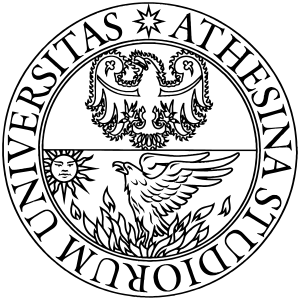
\includegraphics[width=0.3\textwidth]{logo.png}
\end{figure} % Include a department/university logo - this will require the graphicx package
 
%----------------------------------------------------------------------------------------
%	HEADING SECTIONS
%----------------------------------------------------------------------------------------

\textsc{\LARGE UNIVERSITY OF TRENTO}\\[1.3cm] % Name of your university/college
\textsc{\Large Department of Industrial Engineering}\\[0.7cm] % Major heading such as course name
\textsc{\Large Master in Autonomous Systems }\\[0.6cm] % Minor heading such as course title
\textsc{\large Distributed Systems for Measurement and Automation }\\[0.5cm] % Minor heading such as course title

%----------------------------------------------------------------------------------------
%	TITLE SECTION
%----------------------------------------------------------------------------------------

\HRule \\[0.4cm]
{\huge \bfseries Distributed ORCA applied in Simulation of Drones}\\[0.4cm] % Title of your document
\HRule \\[1.3cm]
 
%----------------------------------------------------------------------------------------
%	AUTHOR SECTION
%----------------------------------------------------------------------------------------

\begin{minipage}{0.4\textwidth}
\begin{flushleft} \large
\emph{Authors:}\\
Matteo \textsc{Tadiello} % Your name
\end{flushleft}
\end{minipage}
~
\begin{minipage}{0.4\textwidth}
\begin{flushright} \large
\emph{Supervisor:} \\
Daniele \textsc{Fontanelli, DII} % Supervisor's Name
\end{flushright}
\end{minipage}\\[2cm]

% If you don't want a supervisor, uncomment the two lines below and remove the section above
%\Large \emph{Author:}\\
%John \textsc{Smith}\\[3cm] % Your name

%----------------------------------------------------------------------------------------
%	DATE SECTION
%----------------------------------------------------------------------------------------
{\large \today}\\[0.5cm] % Date, change the \today to a set date if you want to be precise


%----------------------------------------------------------------------------------------

\vfill % Fill the rest of the page with whitespace

\end{titlepage}

\section{Introduction and Objectives}

The Unnamed Aerial Vehicles (\textbf{UAVs}) or drones are becoming more and more used in different applications. The possibility to have a bird view of the world is very useful in many scenarios and the possibility to reach easily space that for a man is difficult or risky are two of the possible application of drones. However a single drone has some limitation due for example to the difficulty to carry heavy objects during fly. This and others problems can be solved using a cooperative swarm of drones or robot, but due to the cooperation of different agents income also different problems as for instance the possibility of collision between different robots. In this writing I present a solution of the problem o the collision between agents using the \textbf{ORCA} approach and testing it in virtual environment with the simulator \textbf{Gazebo}. I will present in order the model used, the solution proposed (ORCA algorithm), the communication system, the implementation of the system and finally the results, ending with the possible improvements and the conclusions.

\section{Model of the Drone}
The Model of the drone is a SDF file explaining the mesh, the collision shape, the inertia matrix and the plugin of each component of the drone. Each drone use the same model template and it contains the following information:
\begin{itemize}[noitemsep,nolistsep]
  \item Drone base link: this is the base structure of the drone where the blades are linked. It's composed by a mesh developed in blender, the inertial component where are described the inertia matrix of the link and it's mass, the collision shape that is been simplified as a box that cover the entire model and a contact sensor and a personalized script that elaborate the contact of each drone. 
  \item The propellers link: four links each one composed by a mesh developed in blender, the inertial component of the propeller that contains the inertia matrix and the mass, the collision shape that is been simplified as a cylinder that cover the propeller.
  \item The propellers joint: four revolute joints that are used for connect each propeller to the base.
  \item The plugin: it contains the functioning of the model and the collision avoidance algorithm.  
\newline 
\end{itemize}
The meshes used for the visualization of the drone are been simplified in order to have as less as possible points in order to improve the final simulation. The same idea is used for the collisions shape that are been thought as simple shapes.
As we can see in the figures \ref{fig:1} and \ref{fig:2}. 

\begin{figure}
\centering
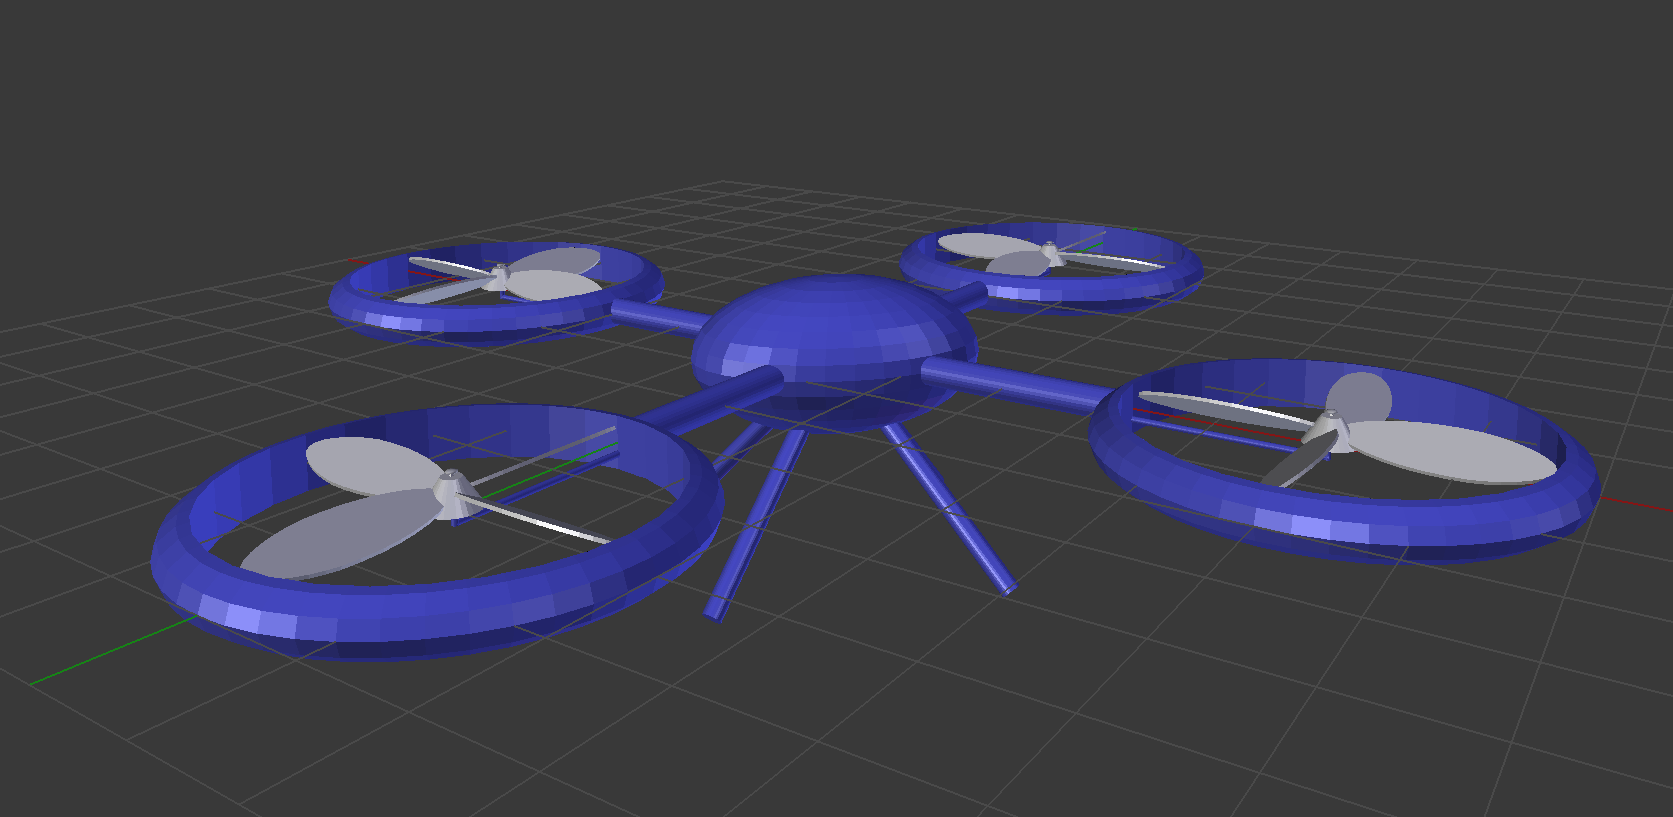
\includegraphics[scale=0.12]{drone.png}
\caption{Mesh of the drone without decreasing number of triangles. }
\label{fig:1}
\end{figure}

\begin{figure}
\centering
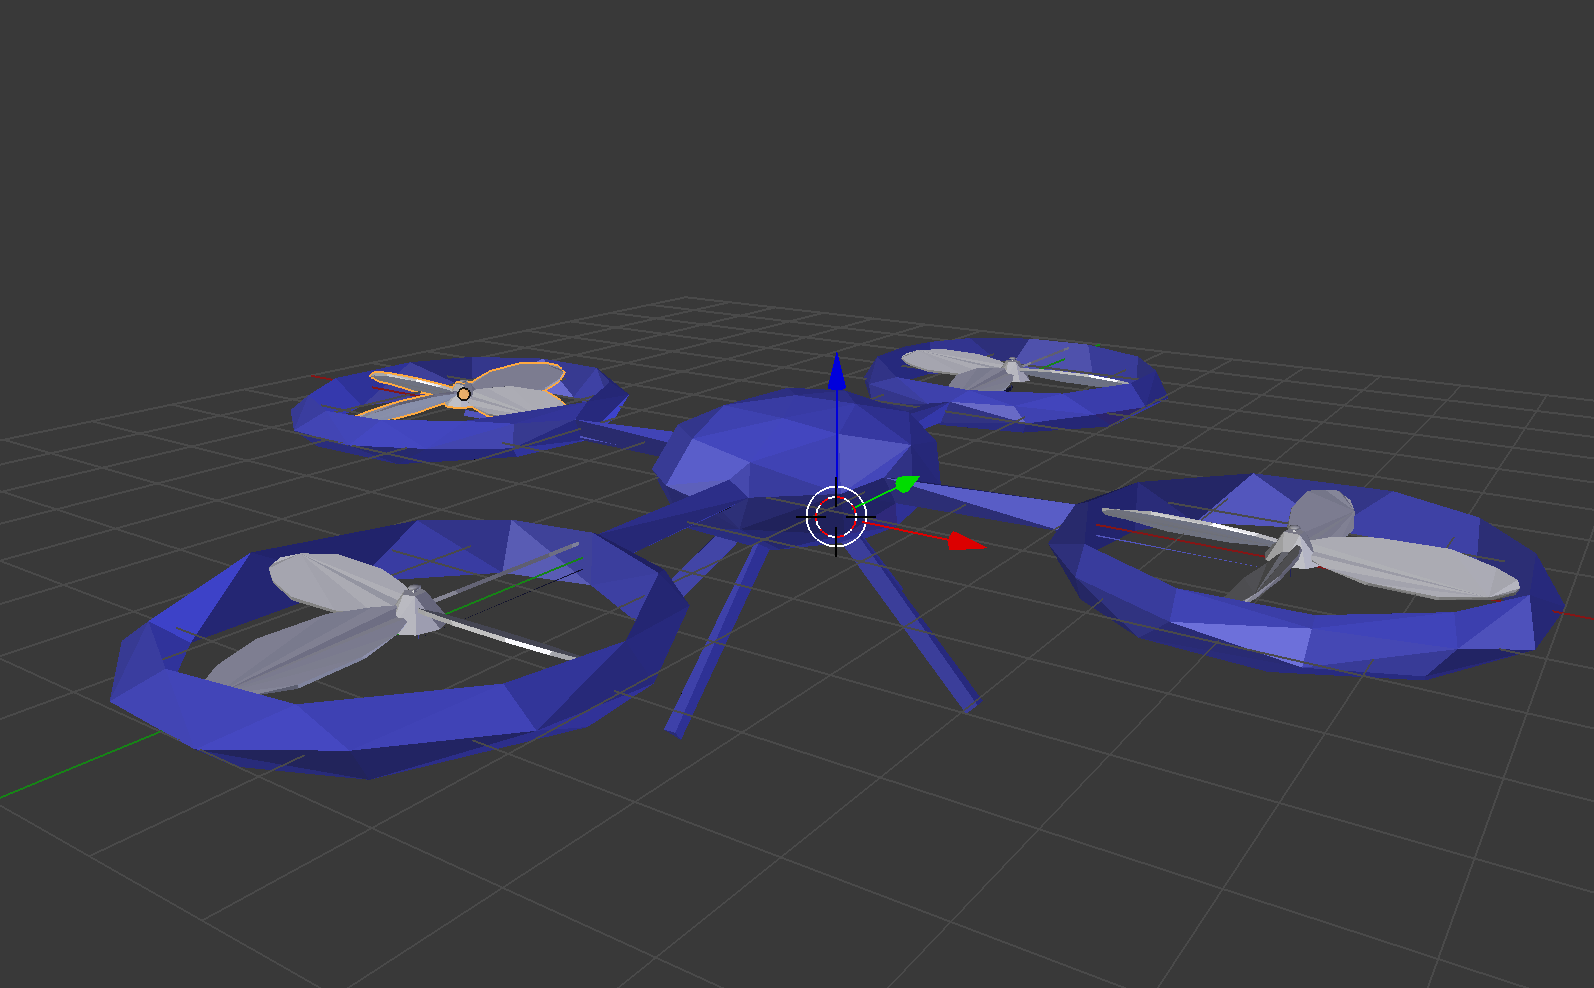
\includegraphics[scale=0.12]{droneSimple.png}
\caption{Mesh of the drone decreased number of triangles. }
\label{fig:2}
\end{figure}

\section{Solution proposed: ORCA Algorithm}
\label{sec:collision avoidance}
The approach chosen to solve this problem is \textbf{Optimal Reciprocal Collision Avoidance ($\mathit{ORCA}$)} \cite{DBLP:conf/dars/Alonso-MoraBRBS10}. The ORCA collision avoidance provide an algorithm that work well in a distributed system because each agent can compute the needed information in autonomy. The main important thing to pay attention is the creation of a good communication system that allow each drone to have the information needed in time to the computation of the action to take.
\\
ORCA is formal approach for reciprocal collision avoidance for robots that have to work in a common work-space. This formulation expect that each drone is completely autonomous and the only essential information needed for the collision avoidance are the position and the velocity of the other elements in the same work-space. The calculation of all the necessary conditions are done in few milliseconds and that approach can be used in crowded spaces. For simplicity I am going to explain the approach in a two dimension environment but in the simulation is used the three dimension algorithm.

\subsection{Formal definition of the problem}
The robots are simplified as followed:
\begin{itemize}
\item simple shape as a circle or a polygon;
\item each agent can move in any direction;
\item the movement is controlled by a velocity vector;
\item it uses ideal sensors, \textit{ i.e.} it knows shape, position and exact velocity of each robot in the environment. 
\end{itemize}
\par
Each robot $A$ has a position $p_A$, a current velocity $v_A$ and a radius $r_A$. These parameter are known or can be perceived by the others agents. Moreover it has a maximum velocity $v^{max}_A$ and a preferred velocity $v^{pref}_A$ (velocity applied if there are not others robot in the environment). This last two parameters are not known by the others.
\par
Each element in the system need to find a new velocity $v^{new}$ for itself in order to achieve the non collision for a time  \(\tau\) preset. As secondary goal the robot has to select the $v^{new}$ as similar as possible at the preferred velocity $v_A^{pref}$.

\subsection{Reciprocal Collision Avoidance}

Given two robot $A$ and $B$ the  \textit{velocity obstacle} $ VO_{A|B}^\tau$ is the set of all the relative velocities of A in respect to B that will bring to a collision in some instant before $t_{now}+\tau$. It is defined as follow:\\
Given D(p,r) a disk with radius $r$ and center $p$;

\begin{equation}
D(p,r) = \{q|\  ||q-p|| < r\}
\end{equation}
therefore
\begin{equation}
VO_{A|B}^\tau= \{v \ |\ \exists t \in [0,\tau ] :: \textit{t}\textbf{v}\in D(p_B - p_A , r_A+r_b)\}
\end{equation}
Are $v_a$ and $v_b$ the actual velocities of the two robots. The definition of \textit{velocity obstacle} involves that if $v_A-v_B \in VO_{A|B}^\tau$, then $A$ and $B$ will collide if the keep the actual velocity, otherwise if $v_A - v_B \notin VO^\tau_{A|B}$ then they will not collide at least until $t_{now}+\tau$. More general, are $X \oplus Y$ the Minkowsky summation of the sets $X$ and $Y$;

\begin{equation}
X \oplus Y = \{ x + y  |  x \in X , y \in Y\},
\end{equation}
then for each set $V_B$, if $v_B \in V_B$ e $v_A \notin VO_{A|B}^\tau \oplus V_B$ then we are sure that until $t_{now}+\tau$ $A$ and $B$ will not collide. Therefor the collision avoidance velocities set $CA^\tau_{A|B}(V_B)$ for $A$  is: 
\begin{equation}
CA_{A|B}^\tau(V_B) = \{ v |  v \notin VO_{A|B}^\tau \oplus V_B \}
\end{equation}
We can now consider that the couple of velocities set $V_A$ and $V_B$ is collision avoiding if $V_A \subseteq CA_{A|B}^\tau (V_B)$ and $V_B \subseteq CA^\tau_{B|A} (V_A)$. In particular if $V_A = CA^\tau_{A|B}(V_B)$ and reciprocally $V_B$ then we can call the two sets \textit{mutually maximal
}.

\subsection{Optimal Reciprocal Collision Avoidance}

Given the definition described above we have to take the velocities sets for $A$ and $B$ such that they are reciprocal collision avoiding at least until $t_{now}+\tau$. Moreover $A$ and $B$ have to reduce their possible optimal velocities to choose without communicate with the others. The couples that optimize these values are denoted as $\mathit{ORCA}^\tau_{A|B}$ and  $\mathit{ORCA}^\tau_{B|A}$ for $B$ and they are defined as:
\par
$\mathit{ORCA}^\tau_{A|B}$ and $\mathit{ORCA}^\tau_{B|A}$ need to be collision avoiding and mutually maximal i.e. $CA^\tau_{A|B}(\mathit{ORCA}^\tau_{B|A}) = \mathit{ORCA}^\tau_{A|B}$ and $CA^\tau_{B|A}(\mathit{ORCA}^\tau_{A|B})=\mathit{ORCA}^\tau_{B|A}$, and for each other collision avoiding velocities set couple $V_A$ and $V_B$ and for each radius $r>0$,
\begin{equation}
  \begin{split}
  |\mathit{ORCA}^\tau_{A|B} \cap D(v_A^{opt}, r )| = |\mathit{ORCA}^\tau_{B|A} \cap D(v^{opt}_B,r)| \\
      \geq min(|V_A \cap D(v_A^{opt},r)|,|V_B \cap D(v_B^{opt},r)|).
  \end{split} 
\end{equation}
Then we have more possible velocities near to $v_A^{opt}$ and $v_B^{opt}$.
\par
Now suppose that both $A$ and $B$ will follow their optimal velocities and that this bring to a collision in $t_{now} + \tau$. Then both $u$ the vector from $v_A^{opt} -v_B^{opt}$ closer to the extremes of the velocities obstacles:
\begin{equation}
u= (argmin_{v \in \delta VO^\tau_{A|B}} ||v-(v^{opt}_A - v^{opt}_B)||)-(v^{opt}_A - v^{opt}_B)
\end{equation}
and $n$ the outward normal of the extreme of $VO^\tau_{A|B}$ in point $(v_A^{opt}-v_B^{opt})+u$.
Than $u$ is the smallest change of velocity for $A$ and $B$ for avoiding the the collision for the next instant. The velocity change is reciprocal so it is expected that $A$ modify his velocity at least of $\frac{1}{2}u$ and $B$ will do the same.
Then the set $\mathit{ORCA}^\tau_{A|B}$ of the velocities allowed for $A$ is the half plane with direction $n$ starting from the point $v^{opt}_A + \frac{1}{2}u$. i.e.
\begin{equation}
	\mathit{ORCA}^\tau_{A|B}= \{v|(v-(v_A^{opt}+ \frac{1}{2}u))\cdot n \geq 0\}.
\end{equation}
symmetrically for $B$. 

\begin{figure}

\centering

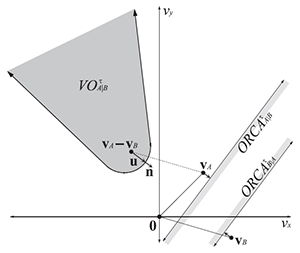
\includegraphics[scale=0.7]{ORCA-1.png}

\caption{The set $\mathit{ORCA}^\tau_{A|B}$ of the allowed velocity of  $A$ for the \textit{optimal reciprocal collision avoidance} with $B$ it is a half-plane delimited by a perpendicular line to $u$  through the point $v^{opt}_A+\frac{1}{2}u$, where the vector from $v^{opt}_A - v^{opt}_B$ to the closest point of the edge of $\mathit{VO}^\tau_{A|B}$.}\label{fig:3}

\end{figure}

\subsection{$n$-Body Collision Avoidance}
For the n-Body Collision Avoidance each root $A$ is in loop of acquiring information and actuation with a time step of $\Delta t$. At each iteration the robot acquire radius, position, and velocity of the others entities and it calculate the half-plane of the velocities for any other robot $B$. The allowed velocities set for $A$ is then the intersection of all the half-plane and it is called $\mathit{ORCA}^\tau_A$. Then $A$ select the velocity closer to the preferred one from $\mathit{ORCA}^\tau_A$. Then the robot reach the new position $p^{new}_A = p_a + v_A^{new}\Delta t$ and the next iteration starts.
They key point of this algorithm is that we need to computer the new velocity in time. This can be achieved using linear programming,  $\mathit{ORCA}^\tau_A$ is a convex region delimited by linear edges. The function to e optimized is the distance to the preferred velocity $v^{pref}_A$. The algorithm as a computational time of $O(n)$, where $n$ is the umber of agents in the system. 

\section{Communication System}
The communication system chosen is a full connect network between all the nodes of the system. The protocol used is UDP this was chosen because the system it's able to work also without the information of all the others drone and it was preferred to have an high number of throughput instead of the security to receive all the message of the system. Each agent collect all the information of the other drones in an array where the information of each agent are stored and it will update whenever a new message from a specified drone is available. Practically each agent create a socket as client and a socket as server. The client is in charge to send the information to all the others agents in the system and the server is in charge to receive the information from all the others agents. The information are updated whenever a message it's received and if a message is lost the new message will provide the information needed for the execution of the algorithm. \\
The simulation system that runs in single machine has create some constraint to the communication system. The communication is run in the same IP address and only the port change from one model to another. That allows the simulation to run properly in a single machine. In real scenario environment probably the communication will be provided with a WiFi module in this case the only setting to change is to modify the IP of each agent instead of the port. The communication via WiFi probably create also a lost of messages higher but it is caused especially to the distance in this case if we don't receive messages from a too distant drone is not a big problem because it's difficult that a drone far away from the receiver will cause a collision.\\
The message sent is a simple struct of double where are stored the following information:
\begin{itemize}
\item An integer \verb|src| that contains the drone that has sent the message;
\item An integer \verb|id| that contains the number of the message sent by the src drone (not used in this simulation because we are sure to don't lost messages);
\item A boolean \verb|sync| for the synchronization between the drones (it's used to say when a drone is ready to move);
\item Three double \verb|x y z| for the pose of the src drone;
\item Three double \verb|Vx Vy Vz| for the velocity of the src drone;
\end{itemize}

\section{System Implementation}
The simulator chosen was Gazebo \cite{gazebo}, It is good for the simulation of robots and their program and algorithms. It allows the generation of realistic ambient. It allows to simulate a population of robot without missing a realistic physics engine and the capacity of visualize the simulation in a graphic environment.
The implementation is started with the creation of the blender meshes that was the base of the model for the simulation. All the component are built in blender with a particular attention on the computational power needed to elaborate that meshes during the simulation. Both the drone's base and the propeller meshes are exported as .dae or .obj in order to be loaded in the gazebo environment. Than was built the .sdf model template as described above. Considering that each drone has singular proprieties as for example the final destination or the IP address a script for the generation of each model was written. This python script allow the generation of different models given the number of drones wanted in the final simulation.    

\section{Experiments and results}

\newline

\begin{figure}[ht!]
\centering
\includegraphics[width=0.4\textwidth]{rssi-test25.jpg}
\caption{Picture taken by the camera of the RSSI setup.The purple dot represents where the kalman filter thinks the robot is (frequently the dot is outside the frame).}
\label{rssi-test25.jpg}
\end{figure}

\begin{figure}[ht!]
\centering
\includegraphics[width=0.5\textwidth]{yposwifi.jpg}
\caption{Example of data got by Kalman filter of RSSI and IMU while the robot was still.}
\label{yposwifi.jpg}
\end{figure}

\begin{figure}[ht!]
\centering
\includegraphics[width=0.3\textwidth]{frame71.jpg}
\caption{Picture of the shape detection got by the OpenCV algorithm. The purple dot shows where the Kalman filter thinks the robot is.}
\label{frame71.jpg}
\end{figure}

\begin{figure}[ht!]
\centering
\includegraphics[width=0.5\textwidth]{xpos1robot.jpg}
\caption{Example of data got by Kalman filter of Camera and IMU while the robot is moving randomly on the frame (x position).}
\label{xpos1robot.jpg}
\end{figure}

\section{Conclusion: limitations and considerations}
In conclusion, the project had some position outcomes and some things which could be done differently. First of all, using only the IMU for localization is not a very good idea, since it has been shown that its variance is too high to have a proper utilization of its data in the fusion. So, for instance, coupling the IMU with some rotary encoders for the wheels would have yielded much greater results.\newline
It can be said that there are some limitations which caused the overall results to be not as good as could have been. From a hardware point of view, the Raspberry Pi lacked the computational ability to deal with the computer vision at a real time rate, this can be seen in the videos, in contrast to this, the real world data which was attained and plotted in graphical form shows that indeed the Kalman filter was working well. The camera however, which has the capability to capture frames at 60 FPS, could not complete its loop cycle in 1/60 seconds, thus the lag is present in the videos.\newline
Overall, the solution has proven it can work, in the future more robots could be added to perform more complex simulations, or other sensors (for example other cameras to grow the robot's work area). 

\bibliographystyle{plain}
\bibliography{references}
\end{document}
